\documentclass[a4paper]{article}
% generated by Docutils <http://docutils.sourceforge.net/>
\usepackage{cmap} % fix search and cut-and-paste in Acrobat
\usepackage{ifthen}
\usepackage[T1]{fontenc}
\usepackage[utf8]{inputenc}
\usepackage{color}
\usepackage{graphicx}

%%% Custom LaTeX preamble
% PDF Standard Fonts
\usepackage{mathptmx} % Times
\usepackage[scaled=.90]{helvet}
\usepackage{courier}

%%% User specified packages and stylesheets

%%% Fallback definitions for Docutils-specific commands

% admonition (specially marked topic)
\providecommand{\DUadmonition}[2][class-arg]{%
  % try \DUadmonition#1{#2}:
  \ifcsname DUadmonition#1\endcsname%
    \csname DUadmonition#1\endcsname{#2}%
  \else
    \begin{center}
      \fbox{\parbox{0.9\linewidth}{#2}}
    \end{center}
  \fi
}

% title for topics, admonitions, unsupported section levels, and sidebar
\providecommand*{\DUtitle}[2][class-arg]{%
  % call \DUtitle#1{#2} if it exists:
  \ifcsname DUtitle#1\endcsname%
    \csname DUtitle#1\endcsname{#2}%
  \else
    \smallskip\noindent\textbf{#2}\smallskip%
  \fi
}

% hyperlinks:
\ifthenelse{\isundefined{\hypersetup}}{
  \usepackage[colorlinks=true,linkcolor=blue,urlcolor=blue]{hyperref}
  \usepackage{bookmark}
  \urlstyle{same} % normal text font (alternatives: tt, rm, sf)
}{}

%%% Body
\begin{document}

Coursework One Results by Zhansultan

\begin{description}
\item[{function Mean results:}] \leavevmode 
1.164  3.916  0.448  5.679  4.865  3.778  4.127  3.604  0.217

\item[{function Covariance results:}] \leavevmode 
5.880  0.245 -0.004 -0.284 -0.346 -0.417 -0.481 -0.267 -0.067
0.245  7.572  0.073 -0.358 -0.346  0.257  2.273  0.946 -0.032

\end{description}

\DUadmonition[system-message]{
\DUtitle[system-message]{system-message}


{\color{red}WARNING/2} in \texttt{Results2.rst}, line~9

Definition list ends without a blank line; unexpected unindent.
backrefs: }

-0.004  0.073  0.247 -0.116 -0.039 -0.003  0.100  0.066 -0.005
-0.284 -0.358 -0.116 16.960  7.969  4.443 -1.036 -0.306  0.047
-0.346 -0.346 -0.039  7.969  8.361  4.921 -0.763 -0.752 -0.001
-0.417  0.257 -0.003  4.443  4.921  6.683 -0.087 -0.376 -0.141
-0.481  2.273  0.100 -1.036 -0.763 -0.087 20.583  1.122  0.014
-0.267  0.946  0.066 -0.306 -0.752 -0.376  1.122  4.317  0.119
-0.067 -0.032 -0.005  0.047 -0.001 -0.141  0.014  0.119  0.170

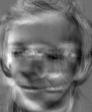
\includegraphics[scale=0.500000]{PrincipalComponent0.jpg}

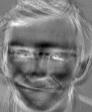
\includegraphics[scale=0.500000]{PrincipalComponent1.jpg}

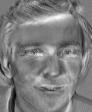
\includegraphics[scale=0.500000]{PrincipalComponent2.jpg}

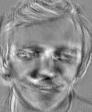
\includegraphics[scale=0.500000]{PrincipalComponent3.jpg}

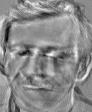
\includegraphics[scale=0.500000]{PrincipalComponent4.jpg}

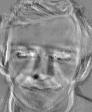
\includegraphics[scale=0.500000]{PrincipalComponent5.jpg}

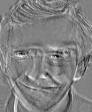
\includegraphics[scale=0.500000]{PrincipalComponent6.jpg}

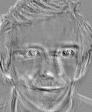
\includegraphics[scale=0.500000]{PrincipalComponent7.jpg}

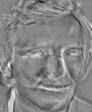
\includegraphics[scale=0.500000]{PrincipalComponent8.jpg}

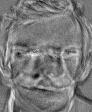
\includegraphics[scale=0.500000]{PrincipalComponent9.jpg}

1206.254 -1590.133 -248.136 -821.249 246.009 -771.900 963.633 376.967 161.599 -533.276

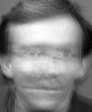
\includegraphics[scale=0.500000]{PartialReconstruction0.jpg}

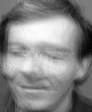
\includegraphics[scale=0.500000]{PartialReconstruction1.jpg}

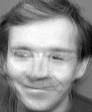
\includegraphics[scale=0.500000]{PartialReconstruction2.jpg}

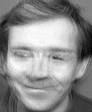
\includegraphics[scale=0.500000]{PartialReconstruction3.jpg}

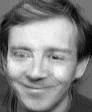
\includegraphics[scale=0.500000]{PartialReconstruction4.jpg}

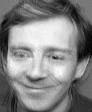
\includegraphics[scale=0.500000]{PartialReconstruction5.jpg}

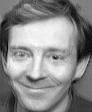
\includegraphics[scale=0.500000]{PartialReconstruction6.jpg}

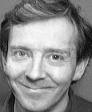
\includegraphics[scale=0.500000]{PartialReconstruction7.jpg}

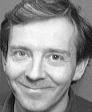
\includegraphics[scale=0.500000]{PartialReconstruction8.jpg}

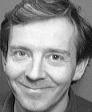
\includegraphics[scale=0.500000]{PartialReconstruction9.jpg}

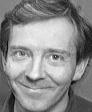
\includegraphics[scale=0.500000]{PartialReconstruction10.jpg}

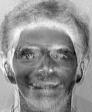
\includegraphics[scale=0.500000]{NewPrincComp0.jpg}

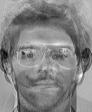
\includegraphics[scale=0.500000]{NewPrincComp1.jpg}

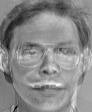
\includegraphics[scale=0.500000]{NewPrincComp2.jpg}

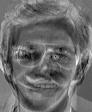
\includegraphics[scale=0.500000]{NewPrincComp3.jpg}

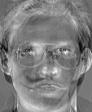
\includegraphics[scale=0.500000]{NewPrincComp4.jpg}

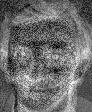
\includegraphics[scale=0.500000]{NewPrincComp5.jpg}

The magnitudes of 'c.pgm' from given basis:
1110.709 1537.080 410.837 -1887.013 941.699 -2009.996

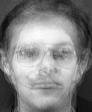
\includegraphics[scale=0.500000]{NewPartRecon0.jpg}

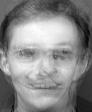
\includegraphics[scale=0.500000]{NewPartRecon1.jpg}

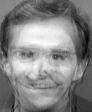
\includegraphics[scale=0.500000]{NewPartRecon2.jpg}

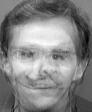
\includegraphics[scale=0.500000]{NewPartRecon3.jpg}

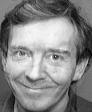
\includegraphics[scale=0.500000]{NewPartRecon4.jpg}

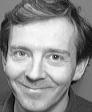
\includegraphics[scale=0.500000]{NewPartRecon5.jpg}

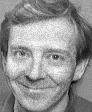
\includegraphics[scale=0.500000]{NewPartRecon6.jpg}

\end{document}
